\documentclass{ximera}  
\title{Loops}  
\begin{document}  
\begin{abstract}  
We give an introduction to for and while loops.
\end{abstract}  
\maketitle

\section{Loops}

Loops are useful whenever you have an algorithm that requires multiple uses of the same step. For example, say we wanted to compute the sum $1+2+\cdots+100$. We have seen in a previous section that this can be done using two variables, one that tracks the current value of the sum and another that tracks whether or not our task is finished (see the flowchart below).

\begin{center}
	    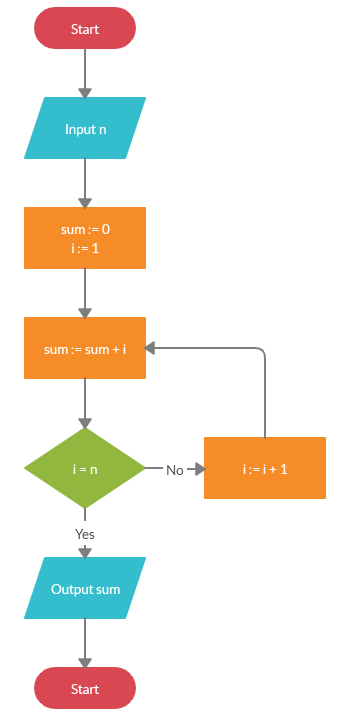
\includegraphics{gausssum2.png}
\end{center}

The structure of the flowchart above is very suggestive of why we use the terminology `loop'. We will now go over two types of loops: for loops and while loops.

\section{For Loops}

The Python syntax for a for loop is as follows:

\begin{verbatim}
==============================

for variable in iterable:
        code

==============================
\end{verbatim}

In the above code, \verb|for| indicates the start of a for loop, \verb|variable| is just a variable name of your choice, \verb|in| is a keyword, and \verb|iterable| is a Python object that can be iterated over, like a list. This Python code almost reads as an English statement. It is saying, for each item in \verb|iterable|, which we will denote by \verb|variable| each time, perform the instructions given by \verb|code|.

Below is an example of how to compute $1+2+\cdots+100$ using a for loop. 

\begin{sageCell}
n = 100
sum = 0

for i in range(1,101):
        sum = sum + i

sum
\end{sageCell}

The \verb|range| function above is commonly used in for loops. The inputs for the \verb|range| function are similar to those used for list slicing. See the SageCells below for examples of how tuse the \verb|range| function.

\begin{sageCell}
# The range function with 1 argument.
for i in range(10):
     print(i)
\end{sageCell}

\begin{sageCell}
# The range function with 2 arguments.
for j in range(2,8):
     print(j)
\end{sageCell}

\begin{sageCell}
# The range function with 3 arguments.
for k in range(3,12,2):
     print(k)
\end{sageCell}

\section{While Loops}



\section{Choices}



\section{Problems}

\begin{question}
\end{question}

\begin{question}
\end{question}

\section{Workspace}

\begin{sageCell}
#
\end{sageCell}

\end{document}
